\documentclass[crop,tikz]{standalone}

\usepackage{amsmath}
\tikzset{>=latex}
\usetikzlibrary{calc,patterns}
\colorlet{green}{black!40!green}
\newcommand{\Fg}{\vec{F}_g}
\newcommand{\vs}{\vec{s}}

\begin{document}
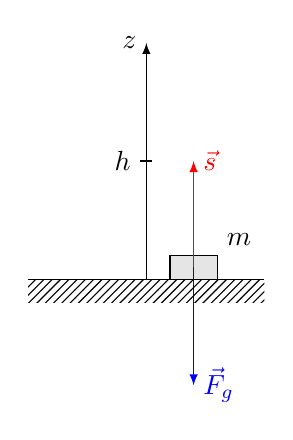
\begin{tikzpicture}[scale=1.5]
  \draw[->] (1,0) -- (1,2) node[left] {$z$};
  \draw[] (0.95,1) node[left] {$h$} -- +(0.1,0);
  \coordinate (K) at (1.4,0.1);
  \draw[fill=gray!20] ($(K)+(-0.2,-0.1)$) rectangle ($(K)+(+0.2,0.1)$) node[above right] {$m$};
  \draw[red,->] (K) -- +(0,0.9) node[right] {$\vs$};
  \draw[blue,->] (K) -- +(0,-1) node[right] {$\Fg$};
  \draw (0,0) -- (2,0);
  \pattern[pattern=north east lines] (0,0)--(2,0)--(2,-0.2)--(0,-0.2)--cycle;
\end{tikzpicture}
\end{document}
